\documentclass[conference]{IEEEtran}
\IEEEoverridecommandlockouts
% The preceding line is only needed to identify funding in the first footnote. If that is unneeded, please comment it out.
%Template version as of 6/27/2024

\usepackage{cite} % Grouping references
\usepackage{amsmath,amssymb,amsfonts} % Math symbols
\usepackage{algorithmic}
\usepackage{graphicx}
\usepackage{textcomp}
\usepackage{xcolor}

% ---- My package ---- %
\allowdisplaybreaks
\usepackage{stfloats}
\usepackage{url}
\usepackage{verbatim}
\usepackage{graphicx}
\usepackage{balance}
\usepackage{array}
%\usepackage{subcaption} % For "pdflatex->bibtex->pdflatex->pdflatex"
\usepackage{algorithm} % Algorithms
\usepackage{caption} % For subfigures (instead of subfig)
\usepackage[labelformat=simple]{subcaption} % For subfigures (instead of subfig)
\renewcommand\thesubfigure{\alph{subfigure}} % For subfigures (instead of subfig)
%\DeclareCaptionLabelFormat{subcaptionlabel}{\normalfont(\textbf{#2}\normalfont)} % For subfigures (instead of subfig) (bold subcaption)
\DeclareCaptionLabelFormat{subcaptionlabel}{\normalfont({#2}\normalfont)} % For subfigures (instead of subfig)
\captionsetup[subfigure]{labelformat=subcaptionlabel} % For subfigures (instead of subfig)

% ---- My newcommand ---- %
\newcommand{\sss}{\scriptscriptstyle}

% ---- My newtheorem ---- %
\newtheorem{proposition}{Proposition}
\newtheorem{lemma}{Lemma}
\newtheorem{theorem}{Theorem}
\newtheorem{corollary}{Corollary}
\newtheorem{definition}{Definition}
\newtheorem{remark}{Remark}


\def\BibTeX{{\rm B\kern-.05em{\sc i\kern-.025em b}\kern-.08em
    T\kern-.1667em\lower.7ex\hbox{E}\kern-.125emX}}


\begin{document}

\title{Secrecy Enhancement and Distributed Architectures in LEO Satellite Networks: A Survey on AN-Assisted Scheduling and SUSDA Design\\
\thanks{This research was partially supported by Basic Science Research Program through the National Research Foundation of Korea(NRF) funded by the Ministry of Education(2021R1I1A3050126).
This research was partially supported by the MSIT(Ministry of Science and ICT), Korea, under the ICAN(ICT Challenge and Advanced Network of HRD) support program(IITP-2025-RS-2022-00156212) supervised by the IITP(Institute for Information \& Communications Technology Planning \& Evaluation).
This work was partially supported by the IITP(Institute of Information \& Coummunications Technology Planning \& Evaluation)-ITRC(Information Technology Research Center) grant funded by the Korea government(Ministry of Science and ICT)(IITP-2025-RS-2024-00437886, 33\%).}
}

\author{\IEEEauthorblockN{Md Sakil Hasan}
\IEEEauthorblockA{\textit{Dept. Mobile Convergence Engineering} \\
\textit{Hanbat National University}\\
Daejeon 34158, the Republic of Korea \\
30224028@o365.hanbat.ac.kr}
\and
\IEEEauthorblockN{Md Gulam Ishak}
\IEEEauthorblockA{\textit{Dept. Mobile Convergence Engineering} \\
\textit{Hanbat National University}\\
Daejeon 34158, the Republic of Korea \\
30251284@o365.hanbat.ac.kr}
\and
\IEEEauthorblockN{Jihwan Moon}
\IEEEauthorblockA{\textit{Dept. Mobile Convergence Engineering} \\
\textit{Hanbat National University}\\
Daejeon 34158, the Republic of Korea \\
anschino@staff.hanbat.ac.kr}
}

\maketitle

%%%%%%%%%%%%%%%%%%%%%%%%%%%%%%%%%%%%%%%%%%%%%%%%%
\begin{abstract}
The rapid deployment of low Earth orbit (LEO) satellite constellations has created new opportunities for high-capacity, low-latency global communication services. However, the broadcast nature of wireless links and the constraints of satellite hardware present unique challenges for ensuring physical-layer security (PLS). At the same time, emerging distributed satellite architectures promise unprecedented flexibility and scalability in cooperative transmission. This survey highlights two complementary research directions that exemplify these trends. First, we review a secrecy outage analysis that introduces an artificial-noise (AN) assisted scheduling strategy in multi-satellite networks. Second, we examine the Spatial Ultra-Sparse Distributed Antenna (SUSDA) architecture in distributed satellite clusters, which leverages laser inter-satellite links, coherent arraying, and adaptive beam synthesis to deliver large-aperture gains, interference suppression, and reconfigurable transmission.
\end{abstract}

\begin{IEEEkeywords}
low Earth orbit (LEO), physical-layer security (PLS), artificial noise (AN), secrecy outage probability(SOP), channel state information (CSI),  artificial noise-assisted satellite scheduling (ANSS), user scheduling, distributed antenna, Distributed Satellite Clusters (DSCs),
\end{IEEEkeywords}


%%%%%%%%%%%%%%%%%%%%%%%%%%%%%%%%%%%%%%%%%%%%%%%%%
\section{Introduction} \label{sec1}

The emergence of large-scale low Earth orbit (LEO) satellite constellations has reshaped the landscape of global communications. Compared with traditional geostationary systems, LEO satellites offer lower latency, higher spatial reuse, and seamless integration with terrestrial networks. These advantages make LEO constellations an attractive platform for supporting broadband Internet access, Internet-of-Things (IoT) connectivity, and mission-critical applications\cite{OKodheli:20}. However, the open nature of wireless propagation combined with the limited hardware resources of small satellites introduces significant challenges in ensuring secure and reliable communications.

Physical-layer security (PLS) has attracted increasing attention as a complementary approach to cryptographic methods. By exploiting channel characteristics such as fading, interference, and noise, PLS enables information-theoretic secrecy without relying solely on computational complexity\cite{PDevi:25}. Among existing techniques, artificial noise (AN) injection and cooperative transmission have shown promise in improving secrecy performance under adversarial conditions\cite{SGoel:08}. Nevertheless, the effectiveness of these methods in LEO satellite networks is shaped by unique factors, including dynamic topology, time-varying channels, and resource constraints.


Covert communication seeks to conceal the presence of a transmission from external detectors, providing low-probability-of-detection protection in addition to confidentiality. This concept has seen growing use in modern wireless systems\cite{SHasan:24}. A widely used technique hides the information signal under AN, allowing the intended receiver to recover it, while NOMA is employed to support covert communications\cite{Chen:23}.

Parallel to security considerations, distributed satellite architectures have emerged as a transformative design paradigm. In particular, spatial ultra-sparse distributed antenna (SUSDA) systems harness multiple satellites flying in close formation to emulate a large-aperture antenna array. Through coherent combining and advanced beam synthesis, SUSDA architectures enhance link quality, suppress interference, and enable flexible reconfiguration\cite{YHe:25}. These capabilities naturally complement PLS strategies by providing new degrees of freedom for secure transmission.

This survey examines two representative research directions that address these issues from complementary perspectives: (i) AN-assisted satellite scheduling for secrecy outage minimization \cite{YLee:25}, and (ii) SUSDA architectures for distributed cooperative transmission \cite{YHe:24}. The scope of the survey is twofold: first, to review the models, assumptions, and findings of each approach; and second, to explore potential synergies and open problems at the intersection of physical-layer security and distributed satellite architectures. By consolidating insights from both works, this survey aims to outline a research agenda for secrecy-aware cooperative transmission in next-generation LEO satellite networks.


%%%%%%%%%%%%%%%%%%%%%%%%%%%%%%%%%%%%%%%%%%%%%%%%%
\section{Background} \label{sec2}

\subsection{Physical-Layer Security in LEO Satellite Networks} \label{sec2.1}

Fifth-generation (5G) and emerging sixth-generation (6G) networks aim to deliver higher data rates, ultra-low latency, and massive connectivity across heterogeneous smart devices while maintaining strong user-data security\cite{SPark:21}.

To protect user and control traffic, the RAN employs standardized ciphering and integrity suites—for example, AES-based 128-EEA2 (LTE) and 128-NEA2 (5G) for encryption, together with integrity algorithms 128-EIA2 (LTE) and 128-NIA2 (5G)—at the appropriate protocol layers, ensuring confidentiality and integrity against interception and eavesdropping\cite{PScalise:24}. Among alternative approaches, physical-layer security (PLS) has attracted growing interest. By leveraging intrinsic channel characteristics, PLS exploits propagation randomness and structure to prevent unauthorized access and reduce susceptibility to eavesdropping\cite{ASanenga:20}.

Recently, satellite-communications research and development have seen renewed focus. As satellite-based wireless services expand, security concerns have intensified because large-scale space information networks are vulnerable to adversarial eavesdropping. Over the past decade, PLS has matured into a complementary protection layer for satellite communications\cite{BLi:20}. In\cite{Talgat:24} investigated PLS for the Low Earth Orbit (LEO)-enabled IoT uplink using a stochastic-geometry framework. It emulated a multi-tier, multi-operator constellation in which satellites acted as legitimate receivers or potential eavesdroppers and incorporated an artificial-noise (AN) scheme via power allocation to quantify the security gains.

Recent studies have examined the secrecy performance of systems that employ a friendly-jammer satellite transmitting AN, while limiting leakage to the legitimate ground user \cite{DNa:25, MHuang:24, IBang:18}. For example, the authors investigated the secrecy performance of a LEO satellite communication system under Nakagami-$m$ fading and proposed a scheme in which a friendly jammer satellite transmits AN toward the eavesdropper while limiting leakage to the legitimate ground user\cite{DNa:25}. In \cite{MHuang:24} a robust secure precoding algorithm for multi-beam satellite non-orthogonal multiple access(NOMA) maximizes the secrecy rate by employing Unmanned Aerial Vehicles (UAVs) transmitting AN to protect legitimate users against eavesdropping. In \cite{IBang:18} the authors proposed a secure user-scheduling scheme for multiuser single-input multiple-output (SIMO) wiretap networks that improved secrecy-outage performance (SOP) and derived closed-form SOP expressions under maximum-ratio combining (MRC) at both the desired receiver and eavesdropper, while operating without instantaneous eavesdropper channel state information (CSI).

We survey the SOP of multi-satellite networks (e.g., LEO constellations) under eavesdropping by jointly scheduling satellites for data transmission and AN injection.

\subsection{Distributed Satellite Architectures and SUSDA} \label{sec2.2}

Distributed Satellite Clusters (DSCs) have emerged as a promising architecture for next-generation non-terrestrial networks (NTNs), addressing the inherent limitations of single-satellite platforms in antenna performance and in-orbit reconfiguration~\cite{PDevi:25}. Building on this concept, the Spatial Ultra-Sparse Distributed Antenna (SUSDA) enables multiple small satellites to form a virtually large, distributed antenna array, thereby enhancing system capacity, strengthening anti-interference capabilities, supporting integrated sensing and communication (ISAC), and relying on enabling technologies such as inter-satellite links, precise synchronization mechanisms, and advanced interference management strategies. Future research is expected to focus on optimizing the performance, efficiency, and scalability of DSC- and SUSDA-based systems.

Beyond terrestrial networks, multi-antenna techniques plays a critical role in satellite communications also, where advanced beamforming enhances link robustness and capacity by precisely directing signals toward targeted regions on Earth~\cite{You:20, Kodheli:20, Heo:23}. These technologies are additionally essential in specialized applications, including radar and navigation for aerospace and maritime sectors, as well as in improving safety for autonomous vehicles and aircraft systems~\cite{Li:07, Li:07_1}.
%%%%%%%%%%%%%%%%%%%%%%%%%%%%%%%%%%%%%%%%%%%%%%%%%
\section{Secrecy in LEO via AN-Assisted Scheduling} \label{sec3}
AN has been widely studied as an effective tool for physical-layer security, particularly in multi-antenna terrestrial networks. Extending this concept to satellite networks, the recent work\cite{YLee:25} has investigated the use of coordinated satellites to transmit data and AN simultaneously. The key idea is to leverage the constellation-wise inherent spatial diversity by assigning one satellite to deliver confidential data while another transmits artificial noise to confuse potential eavesdroppers.

\subsection{System Model} \label{sec3.1}
The considered scenario is illustrated in Figure 1. A LEO satellite transmits data to the ground base station (GBS), while a malicious UAV attempts to eavesdrop on the satellite-to-ground signal. The network comprises a cluster of $M$ LEO satellites, a single GBS, and the UAV eavesdropper. Each satellite is equipped with a single
antenna, whereas the GBS and the UAV employ antennas.

We let $\alpha^\star$ and $\beta^\star$ denote the scheduled-satellite indices for data and AN transmission, respectively. Using linear receive weight vectors, the achievable rates at the GBS and the malicious UAV are given by\cite{YLee:25}:

\begin{align}
r_g &= \log_2\!\left(
  1 + \frac{\lVert \mathbf{w}_g^{\mathrm H}\mathbf{h}_{\alpha^\star} \rVert^{2}}
           {\lVert \mathbf{w}_g^{\mathrm H}\mathbf{h}_{\beta^\star} \rVert^{2} + 1/\rho_g}
\right), \tag{1}\\[2mm]
r_u &= \log_2\!\left(
  1 + \frac{\lVert \mathbf{w}_u^{\mathrm H}\mathbf{s}_{\alpha^\star} \rVert^{2}}
           {\lVert \mathbf{w}_u^{\mathrm H}\mathbf{s}_{\beta^\star} \rVert^{2} + 1/\rho_u}
\right). \tag{2}
\end{align}Here, $\rho_g$ and $\rho_u$ denote the transmit signal-to-noise ratio (SNR),
defined as $\rho_g \triangleq \dfrac{P_T}{\sigma_g^{2}}$ and
$\rho_u \triangleq \dfrac{P_T}{\sigma_u^{2}}$, respectively
The GBS knows the instantaneous CSI via channel estimation, whereas the CSI between the satellite and the UAV is unavailable at the GBS—a realistic assumption under passive eavesdropping \cite{YLee:25}. Hence, the authors in \cite{YLee:25} evaluated secrecy using the SOP rather than the instantaneous secrecy rate, defined as
\begin{equation}
P_{\mathrm{so}}(\tau) \triangleq \Pr\{\, r_g - r_u < \tau \,\}. \tag{3}
\end{equation}where $r_g$ and $r_u$ are given in (1)-(2), and $\tau$ denotes the secrecy rate threshold.

\subsection{AN-Assisted Satellite Scheduling} \label{sec3.2}
The GBS exploits pilot-based downlink CSI to select (i) a data satellite with a strong channel and (ii) an AN satellite whose interference can be mitigated via linear weight vectors at the GBS. Secrecy performance is analyzed under Nakagami-$m$ fading for both single- and multi-antenna receivers at the GBS and a UAV eavesdropper. An algorithm to select the best transmit and AN satellites and optimize the beamforming vector was provided by\cite{YLee:25}. Meanwhile, an alternative algorithm to solve the optimization problem can be designed as in Algorithm~\ref{alg1}.

\begin{algorithm}
  \caption{Artificial Noise-Assisted Satellite Scheduling}
  \begin{algorithmic}[1]
    \STATE $\textbf{Input:}$ $\{\mathbf{h}_1, \mathbf{h}_2, \ldots, \mathbf{h}_M\}$ $\textsf{//a set of channel vectors }$
    \STATE $\textbf{Output:}$ $\alpha^\star\leftarrow 0,$  $\beta^\star\leftarrow 0, $ $\mathbf{w}_g\leftarrow 0, $ $\mu\leftarrow 0$
    
    \FOR{$i \in \left\{1,\ldots,M\right\}$}
      \STATE $i^\star = \arg\min \|\mathbf{h}_i\|$ \textsf{//pick AN satellite candidate}
      
      \STATE Calculate $\mathbf{P}_{i^\star}= \frac{\mathbf{h}_ {i^\star}\,\mathbf{h}_{i^\star}^{\mathrm H}}{\lVert \mathbf{h}_{i^\star} \rVert^{2}}$ \textsf{// Projection matrix }
      \STATE Set $\mathbf{w}_{i^\star}\in svd(\mathbf{P}_{i^\star})$ \textsf{// Nullspace of $\mathbf{h}_{i^\star}$}
      \FOR{$j \in \{1,\ldots,M\}\setminus\{i^\star\}$}
          \IF{$\big\lVert \mathbf{w}_{i^\star}^{\mathrm H}\mathbf{h}_j \big\rVert > \mu$}
            \STATE Update $\alpha^\star \leftarrow j$
            \STATE Update $\mu \leftarrow \big\lVert \mathbf{w}_{i^\star}^{\mathrm H}\mathbf{h}_j \big\rVert$
            \STATE $\mathbf{w}_g \leftarrow \mathbf{w}_{i^\star}$
            \STATE $\beta^\star \leftarrow i^\star$;
          \ENDIF
      \ENDFOR
    \ENDFOR
  \end{algorithmic}
  \label{alg1}
\end{algorithm}

\begin{figure}
  \centering
  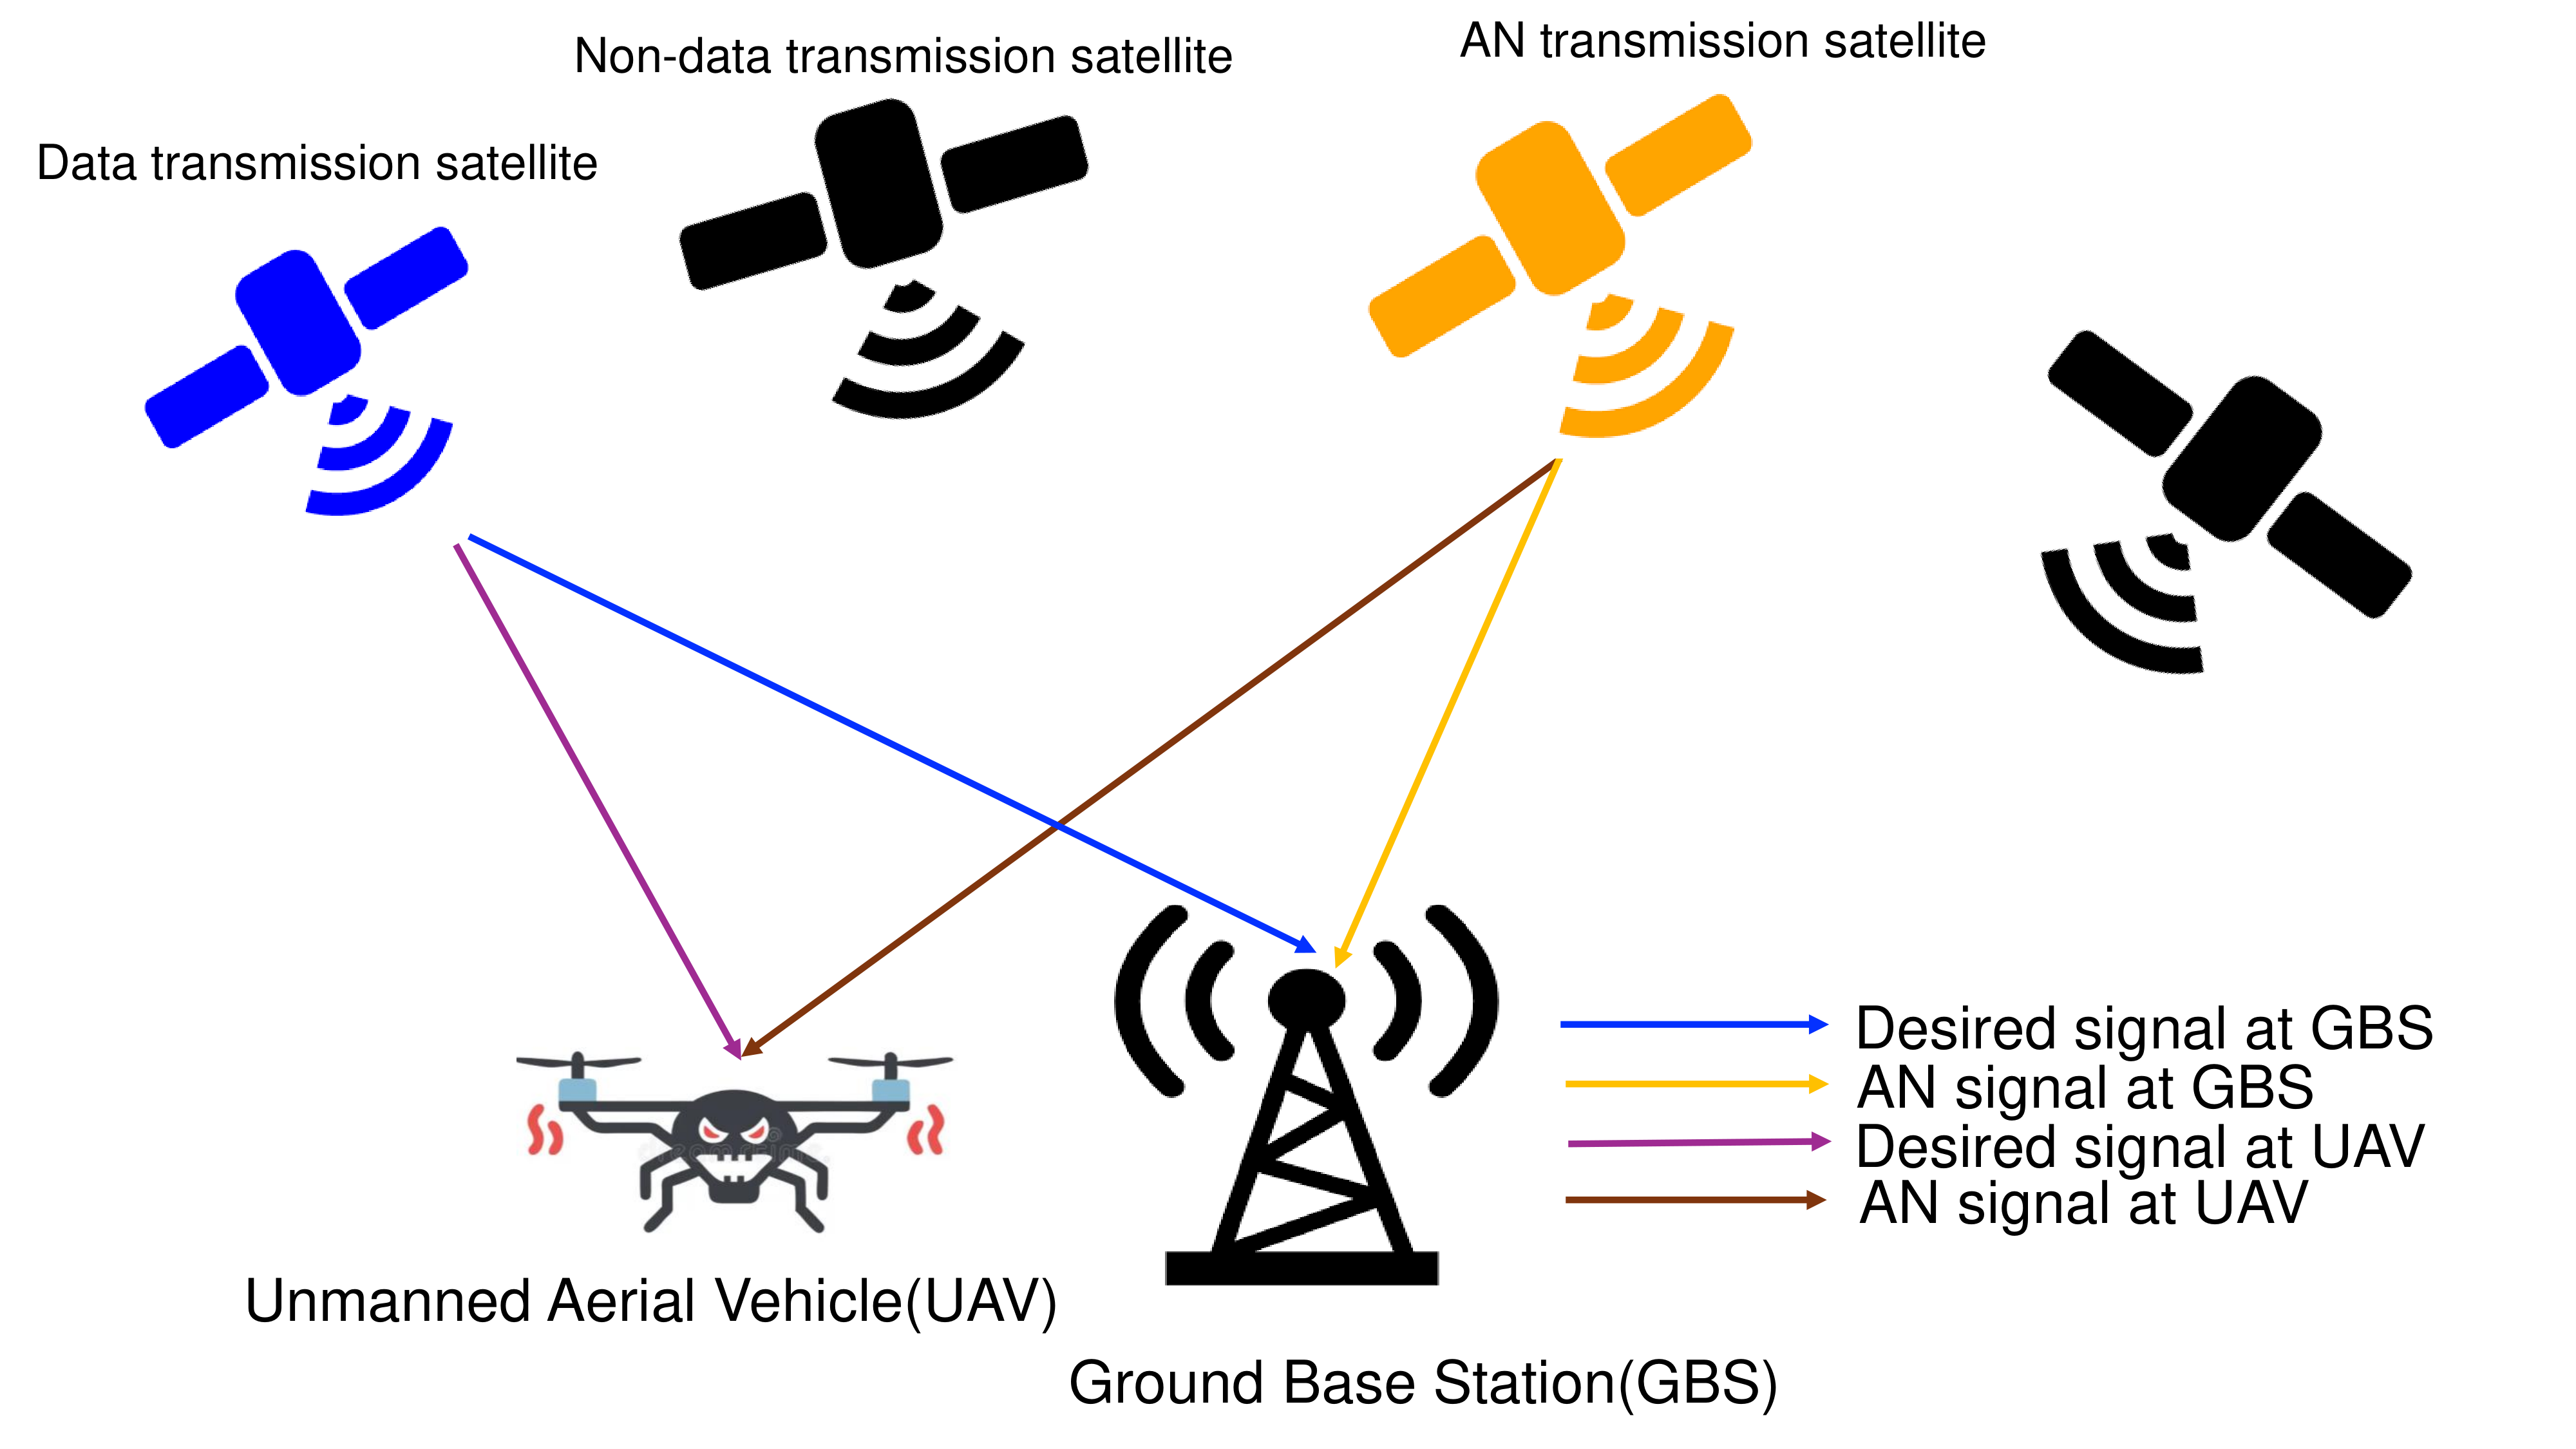
\includegraphics[width=0.47\textwidth]{System_model.png}
  \caption{System model in \cite{YLee:25}}
  \label{fig1}
\end{figure}
In\cite{YLee:25}, Algorithm~\ref{alg1} achieves optimal pair selection for the stated metric at the expense of an $M-$fold increase in nullspace computations and a quadratic inner-product complexity $\mathcal{O}(M^2 n)$, yielding higher latency; by contrast,the above Algorithm\ref{alg1} is a greedy, low-complexity scheduler with per-decision complexity $\mathcal{O}(n^{3})+\mathcal{O}(Mn)$, equires minimal CSI/signaling, and attains lower latency.
\subsection{Secrecy Outage Analysis} \label{sec3.3}
The authors derived a closed-form expression for the SOP under the proposed scheme in the single-antenna case. Using (1) and (2), the final SOP in (2) is rewritten as

\begin{multline}
p_{\mathrm{so}}(\tau)
= M\Bigl(\frac{m^{m}}{\Gamma(m)}\Bigr)^{3}
\sum_{a=0}^{M}\sum_{b=0}^{M}\sum_{d=0}^{M}\sum_{e=0}^{b}
\sum_{i=0}^{m}\sum_{p=0}^{b}\sum_{v=0}^{p-m-i}\\
\times \sum_{q=0}^{\infty}
e^{m\sigma^{2}(a-\lambda)}(-1)^{a+b-p+q}\binom{M}{a}\,\delta_{b,a}\,\beta_t\\
\times {a}^{b+d}\sigma^{2(e+m-i)}
\binom{b}{e}\binom{m}{i}\binom{p-m-i}{v}\\
\times\binom{j+q-1}{q}2^{\tau v} A^{-j-v}\lambda^{v}
\Gamma(m+d+b-e)\\
\times\Gamma(m+i)\frac{\Gamma(m+v+q)}{(m\sigma^{2}(\lambda+1))^{m+v+q}} 
\tag{4}
\end{multline}
where \(j=a+d+b-e,\quad\lambda = a\,2^{\tau},\quad
A=M-a+\lambda\) and ${\sigma^{2}}={\sigma_g^{2}}={\sigma_u^{2}}$ 

The authors in \cite{YLee:25} assumed that each channel coefficient follows Nakagami-$m$ fading. The same shape parameter $m$ is used for both the GBS-satellite and UAV-satellite links, while allowing the scale parameter to differ across the two links. Coefficients within each vector are independent and identically distributed (i.i.d), and the same assumptions apply to all satellites.

\subsection{Key Findings and Limitations} \label{sec3.4}

In\cite{YLee:25} the authors proposed an ANSS scheme that jointly selects one satellite for data transmission and another for artificial-noise injection in LEO networks under Nakagami-$m$ fading. They further derived a closed-form SOP for the single-antenna case. As future work, one may develop real-time, low-complexity variants of AN-assisted scheduling that scale to large constellations. The findings also suggest practical applications, such as a military defense.


%%%%%%%%%%%%%%%%%%%%%%%%%%%%%%%%%%%%%%%%%%%%%%%%%
\section{SUSDA: Capabilities and Challenges} \label{sec4}
Distributed satellite architectures have emerged as a promising solution to overcome the size, weight, and cost limitations of single large-aperture antennas. Among them, the SUSDA concept represents a paradigm shift in constellation design, enabling multiple satellites to operate cooperatively as a large, reconfigurable antenna array.

\subsection{Architectural Overview} \label{sec4.1}
The network architecture appears in Fig. 2. The SUSDA architecture integrates distributed antennas and inter-satellite synchronization to enable coherent multi-satellite beamforming. Small-aperture antennas on DSC satellites form a virtual array, providing high SNR outputs and supporting flexible topologies, including linear, ring, star, or hybrid formations.

In the uplink, ground RF signals are delay-compensated, converted, and shared via inter-satellite links, with cross-correlation ensuring precise synchronization. In the downlink, satellites pre-compensate for geometric delays, allowing ground terminals to recover synchronized signals through phase adjustment and demodulation. This cooperative design enables reliable, high-throughput space-ground connectivity.
\begin{figure}
  \centering
  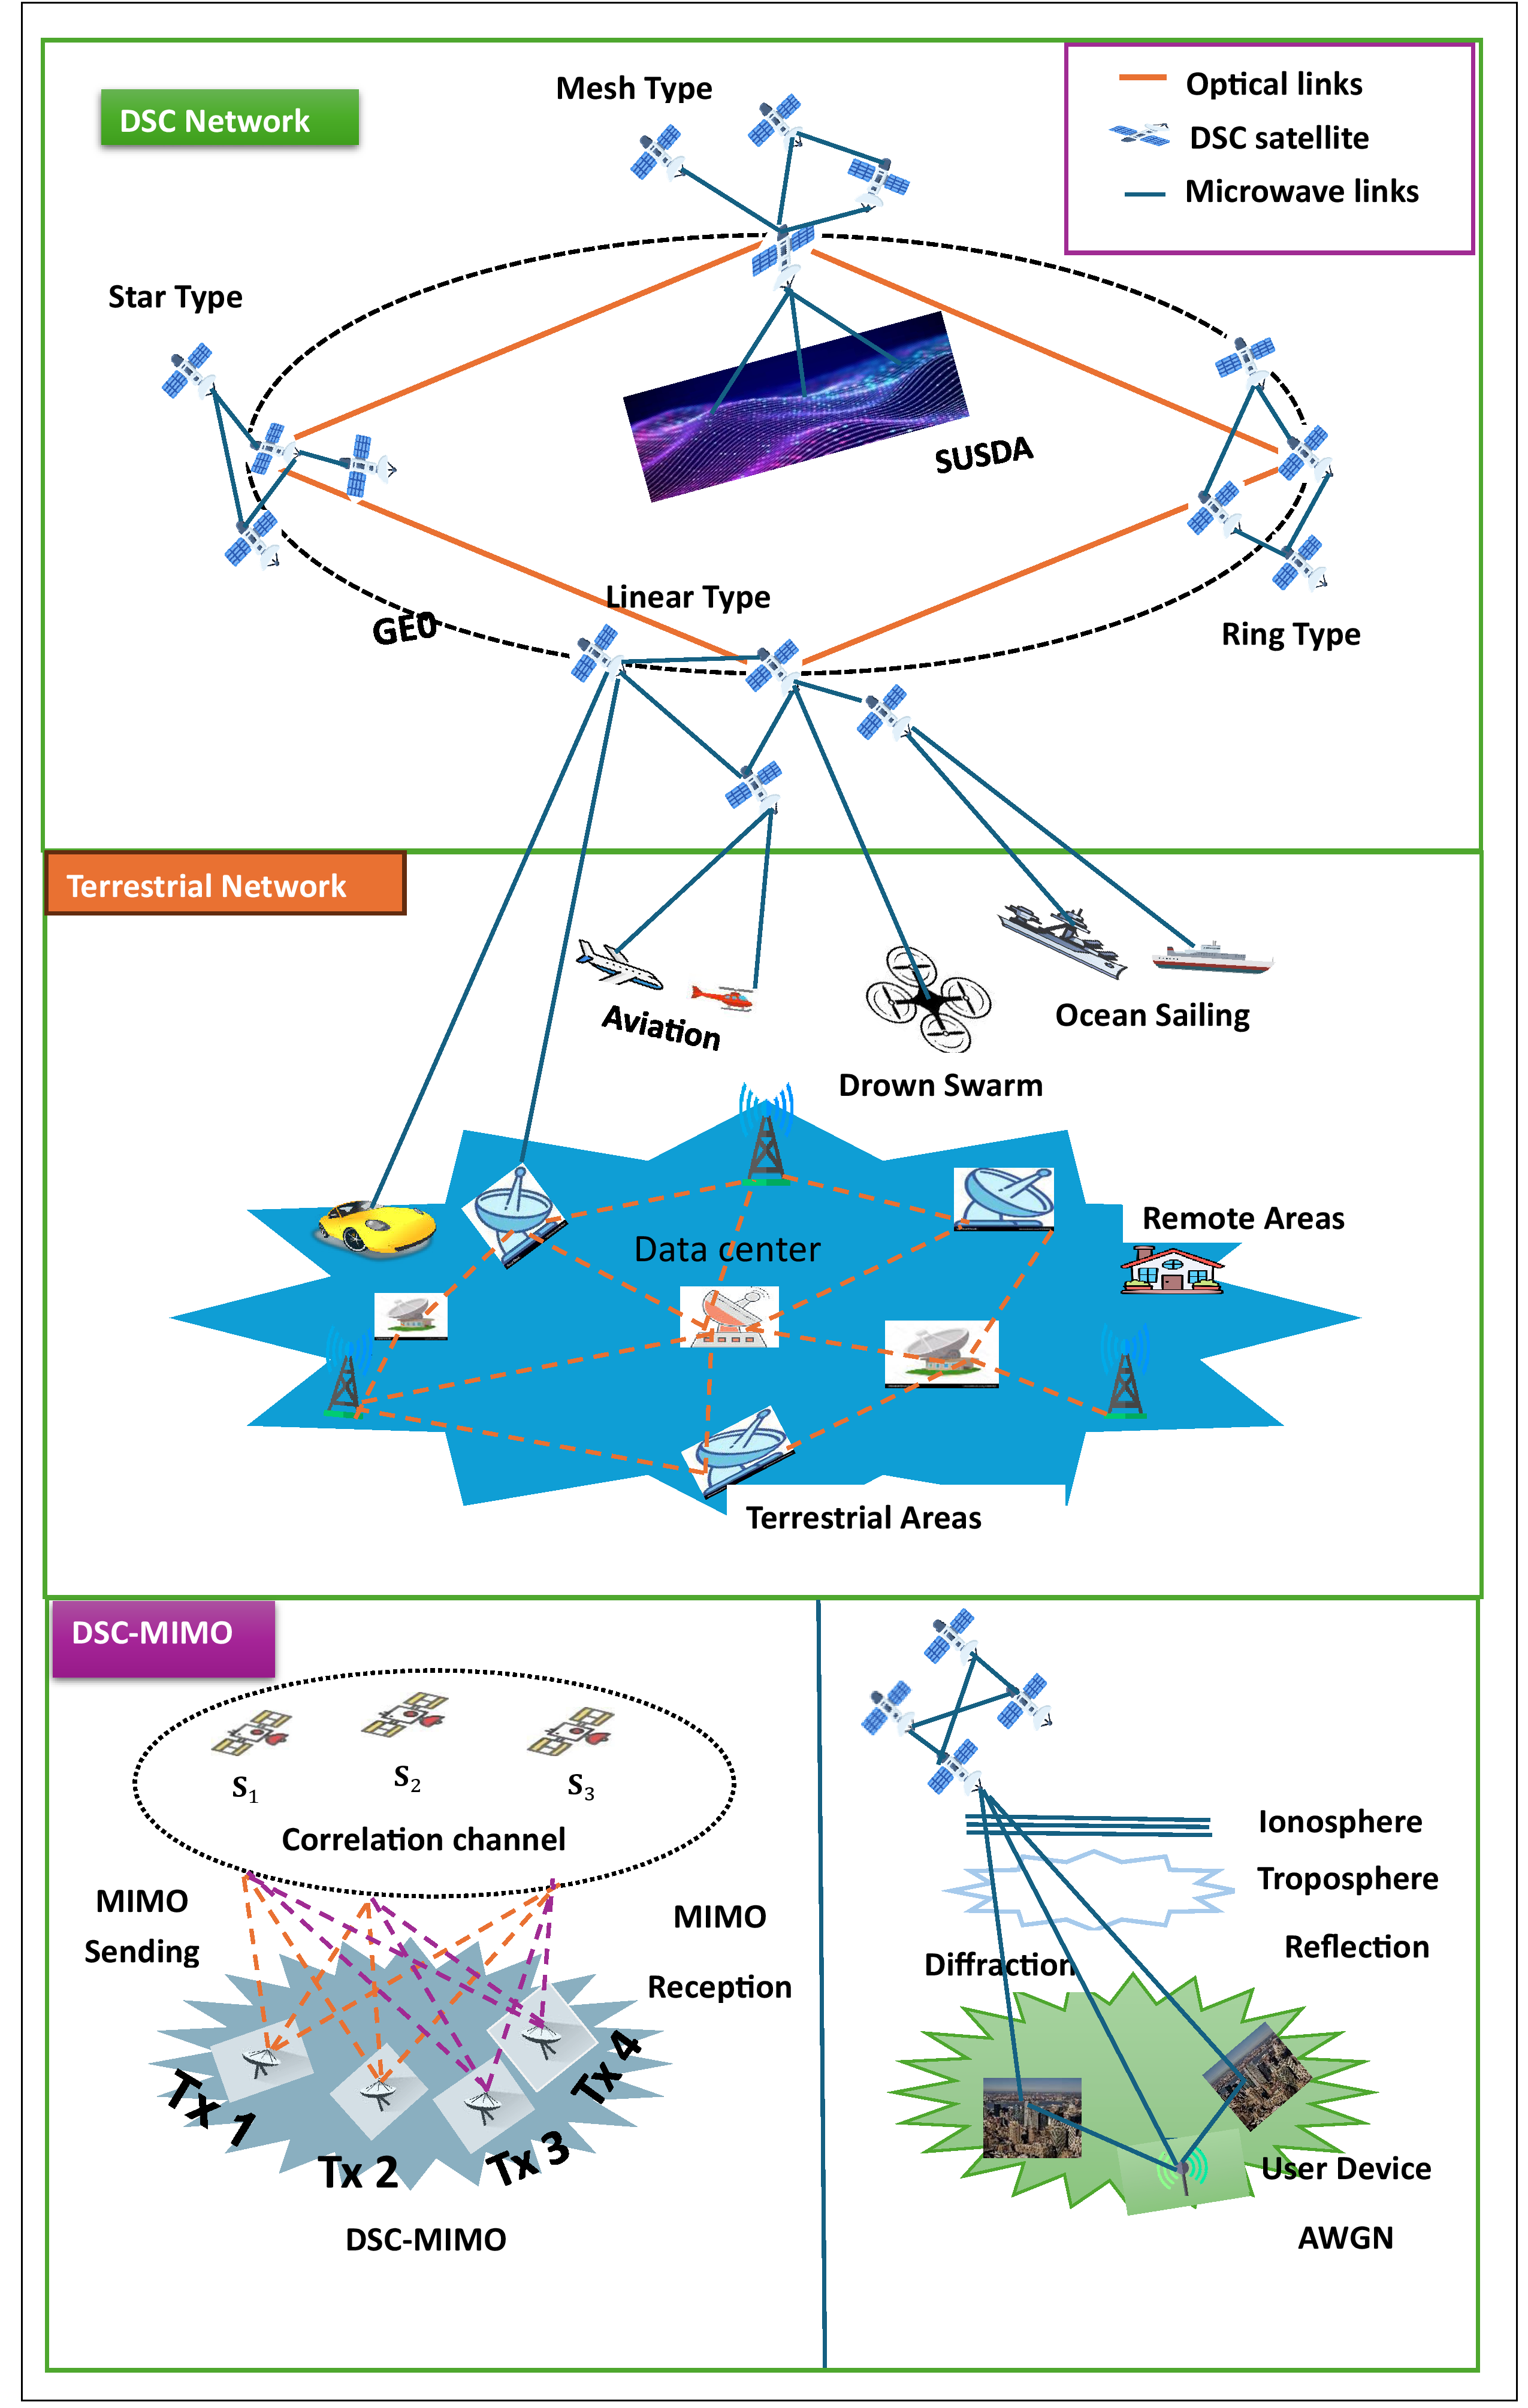
\includegraphics[width=0.47\textwidth]{System_model_2.png}
  \caption{Architecture of SUSDA satellite-ground collaborative transmission in \cite{YHe:24}}
  \label{fig2}
\end{figure}

\subsection{Key Enabling Technologies} \label{sec4.2}
\subsubsection{Inter-Satellite Links (ISLs)} \label{sec4.2.1}
ISLs are crucial for real-time coordination among Distributed Satellite Clusters (DSCs). Optical (laser) ISLs are preferred over microwave due to higher capacity, lower power consumption, and reduced interference; however, challenges such as visibility, connectivity, and antenna size persist. Robust ISLs provide the backbone for delay compensation, synchronization, and distributed processing in SUSDA architectures
\subsubsection{DSC-MIMO Transmission} \label{sec4.2.2}
DSC-MIMO leverages spatial diversity and multiplexing by employing multiple antennas across satellites and ground stations. In the uplink, ground transmitters apply MIMO encoding, satellites forward the signals, and ground receivers perform decoding. This distributed architecture enhances spectral efficiency and provides improved resilience against fading and interference
\subsubsection{Synchronization and Delay Compensation} \label{sec4.2.3}
Precise synchronization is essential due to kilometer-scale satellite spacing. Each DSC node calculates and compensates for geometric delays, with results shared via inter-satellite links (ISLs). Cross-correlation is employed to refine timing and support coherent beamforming. In the downlink, phase-aligned transmissions enable reliable signal recovery, preserving array coherence in dynamic orbital environments

\subsection{Challenges and Design Issues} \label{sec4.3}
\subsubsection{Grating Lobes and Sidelobes} \label{sec4.3.1}
As an ultra-sparse array, SUSDA generates strong grating lobes that reduce antenna gain and degrade localization performance. Mitigation requires non-periodic array configurations and intelligent optimization techniques. Sparse array synthesis methods are employed to suppress grating lobes while maintaining safe inter-satellite spacing

\subsubsection{Channel Modeling} \label{sec4.3.2}
SUSDA channels are affected by mobility-induced fading, multipath propagation, and Doppler shifts. High correlation among satellites constrains both capacity and reliability. Correlated shadowed Rice fading models, along with techniques such as signal diversity, spatial multiplexing, and advanced channel estimation, can be employed to mitigate these effects  
\subsubsection{Adaptive Anti-Interference} \label{sec4.3.3}
Dynamic interference requires adaptive control. SUSDA leverages real-time sensing, beamforming adjustment, and deep reinforcement learning (DRL)-based strategies to optimize anti-interference performance while maintaining service quality, thereby ensuring robust operation under challenging conditions
\subsubsection{Mobility and Integration} \label{sec4.3.4}
Mobility across orbits introduces challenges in synchronization and channel stability. Extending SUSDA to low Earth orbit (LEO) necessitates precise navigation and alignment, whereas integration with geostationary orbit (GEO) satellites provides redundancy. Coupling SUSDA with multi-access edge computing (MEC) platforms enables distributed computation, thereby reducing latency and enhancing system reliability.
\subsection{Research Opportunities} \label{sec4.4}
Future research in satellite communications encompasses several critical areas. Advanced channel modeling and estimation remain essential, as current models cannot fully capture Doppler, multipath, and delay effects in ultra-sparse constellations. Machine learning-driven prediction and hybrid deterministic-stochastic models for GEO, MEO, and LEO channels represent promising directions. Similarly, intelligent grating lobe and sidelobe suppression is necessary, since ultra-sparse arrays generate strong lobes that degrade performance. AI-assisted array design and real-time reconfigurable synthesis could dynamically mitigate lobes and enhance beamforming. Adaptive anti-interference schemes based on deep reinforcement learning (DRL) also show potential but face scalability challenges; future work may explore multi-agent RL, federated learning, and cross-layer AI models to enable robust interference mitigation. Synchronization and delay compensation at scale remain critical, motivating investigations into quantum clock distribution, GNSS-free timing, and joint communication-sensing synchronization to improve system robustness.

Other research directions include the integration of non-terrestrial networks with multi-access edge computing (MEC) and edge intelligence, mobility management in LEO and multi-orbit systems, and the development of novel modulation schemes. Lightweight MEC nodes on satellites possess limited computing power, necessitating energy-aware task scheduling strategies across satellites, GEO relays, and ground stations. LEO expansion further requires stable swarm formation and cross-orbit integration, which may be enabled through swarm intelligence algorithms and standardized multi-orbit protocols. Finally, orthogonal time-frequency space (OTFS) modulation offers strong Doppler resilience but must be integrated with MIMO and multiple access schemes; combining OTFS with NOMA or SCMA may unlock new capabilities for high-mobility 6G non-terrestrial networks.

%%%%%%%%%%%%%%%%%%%%%%%%%%%%%%%%%%%%%%%%%%%%%%%%%
\section{Joint Design Opportunities} \label{sec5}
The two research directions reviewed in this survey—AN-assisted scheduling for secrecy enhancement and SUSDA-based distributed architectures—approach the problem of secure LEO communication from complementary perspectives. While the former develops analytical tools and scheduling strategies to minimize secrecy outage, the latter provides a cooperative physical infrastructure capable of amplifying such techniques. Their integration offers several promising opportunities.

\subsection{Distributed Artificial-Noise Beamforming} \label{sec5.1}
AN-assisted scheduling has demonstrated that even a single AN-transmitting satellite can significantly improve secrecy. Within a SUSDA architecture, multiple satellites could jointly transmit AN in a phase-coherent manner, effectively shaping interference patterns. This would allow the constellation to direct AN energy toward potential eavesdroppers while nulling it at legitimate receivers, thereby extending single-satellite AN strategies into constellation-scale beamforming.

\subsection{Secrecy Outage with Correlated Channels} \label{sec5.2}
The secrecy outage analysis in current AN-assisted schemes assumes independent fading channels. In contrast, SUSDA emphasizes channel correlation across closely spaced satellites. Incorporating correlated fading into secrecy outage probability analysis would yield more realistic performance bounds and could inform optimal satellite spacing and formation design for secrecy enhancement.

\subsection{Robust Scheduling under Synchronization and Delay Constraints} \label{sec5.3}
The AN-assisted scheduling framework assumes perfect CSI at the GBS and negligible coordination delay. SUSDA architectures, however, must contend with synchronization errors, ISL latency, and Doppler dynamics. Extending secrecy-aware scheduling to account for delayed or imperfect CSI would make the framework more robust and practical in distributed satellite clusters.

\subsection{Joint Array Pattern and Security Optimization} \label{sec5.4}
SUSDA research has highlighted the need to suppress grating lobes and optimize sparse array layouts. By integrating secrecy objectives, array synthesis could be extended to jointly minimize sidelobe leakage and maximize secrecy capacity. This would enable simultaneous optimization of communication performance and physical-layer security, aligning with the broader trend of multi-objective constellation design.

\subsection{Learning-Based Security Adaptation} \label{sec5.5}
Both AN-assisted secrecy schemes and SUSDA anti-interference strategies can benefit from machine learning. Reinforcement learning could be applied to dynamically allocate satellites for data versus AN roles, adapt beam patterns under adversarial conditions, and balance tradeoffs between throughput, interference suppression, and secrecy performance.


%%%%%%%%%%%%%%%%%%%%%%%%%%%%%%%%%%%%%%%%%%%%%%%%%
\section{Conclusion} \label{sec6}
This survey has reviewed two complementary research directions addressing these challenges. The first was AN assisted scheduling, which leverages cooperative satellites to minimize secrecy outage probability and demonstrates the potential of constellation-scale diversity for physical-layer security. The second was the SUSDA architecture, which exploits tightly coordinated satellite clusters to emulate large-aperture arrays, enabling coherent combining, interference suppression, and flexible reconfiguration. Together, these approaches highlighted the dual importance of secrecy strategies and distributed architectures in shaping the future of secure LEO networks. Their integration offered promising opportunities such as distributed AN beamforming, secrecy-aware array synthesis, and learning-enabled adaptive security. At the same time, several open problems remain, including multi-antenna secrecy analysis under correlated channels, robust scheduling under imperfect CSI, and geometry-aware secrecy optimization. Looking ahead, the convergence of physical-layer security and distributed cooperative architectures will play a pivotal role in the design of next-generation satellite communication systems. By unifying secrecy objectives with constellation-scale cooperation, future LEO networks can achieve both high capacity and strong resilience against eavesdropping, advancing toward secure and intelligent global connectivity.


%%%%%%%%%%%%%%%%%%%%%%%%%%%%%%%%%%%%%%%%%%%%%%%%%
\bibliographystyle{ieeetr}

\bibliography{AZREF}

\end{document}
